\documentclass[]{article}
\usepackage{lmodern}
\usepackage{amssymb,amsmath}
\usepackage{ifxetex,ifluatex}
\usepackage{fixltx2e} % provides \textsubscript
\ifnum 0\ifxetex 1\fi\ifluatex 1\fi=0 % if pdftex
  \usepackage[T1]{fontenc}
  \usepackage[utf8]{inputenc}
\else % if luatex or xelatex
  \ifxetex
    \usepackage{mathspec}
  \else
    \usepackage{fontspec}
  \fi
  \defaultfontfeatures{Ligatures=TeX,Scale=MatchLowercase}
\fi
% use upquote if available, for straight quotes in verbatim environments
\IfFileExists{upquote.sty}{\usepackage{upquote}}{}
% use microtype if available
\IfFileExists{microtype.sty}{%
\usepackage{microtype}
\UseMicrotypeSet[protrusion]{basicmath} % disable protrusion for tt fonts
}{}
\usepackage{hyperref}
\hypersetup{unicode=true,
            pdfborder={0 0 0},
            breaklinks=true}
\urlstyle{same}  % don't use monospace font for urls
\usepackage{longtable,booktabs}
\usepackage{graphicx,grffile}
\makeatletter
\def\maxwidth{\ifdim\Gin@nat@width>\linewidth\linewidth\else\Gin@nat@width\fi}
\def\maxheight{\ifdim\Gin@nat@height>\textheight\textheight\else\Gin@nat@height\fi}
\makeatother
% Scale images if necessary, so that they will not overflow the page
% margins by default, and it is still possible to overwrite the defaults
% using explicit options in \includegraphics[width, height, ...]{}
\setkeys{Gin}{width=\maxwidth,height=\maxheight,keepaspectratio}
\IfFileExists{parskip.sty}{%
\usepackage{parskip}
}{% else
\setlength{\parindent}{0pt}
\setlength{\parskip}{6pt plus 2pt minus 1pt}
}
\setlength{\emergencystretch}{3em}  % prevent overfull lines
\providecommand{\tightlist}{%
  \setlength{\itemsep}{0pt}\setlength{\parskip}{0pt}}
\setcounter{secnumdepth}{0}
% Redefines (sub)paragraphs to behave more like sections
\ifx\paragraph\undefined\else
\let\oldparagraph\paragraph
\renewcommand{\paragraph}[1]{\oldparagraph{#1}\mbox{}}
\fi
\ifx\subparagraph\undefined\else
\let\oldsubparagraph\subparagraph
\renewcommand{\subparagraph}[1]{\oldsubparagraph{#1}\mbox{}}
\fi

\date{}

\begin{document}

\section{ParallelGeneticsInspiredNeuralNetworkTuning}\label{parallelgeneticsinspiredneuralnetworktuning}

\subsection{Introduction:}\label{introduction}

The first analysis for optimizing neural network is shown
\href{https://github.com/bhatnags/GeneticsInspiredNeuralNetworkTuning}{here}.
Keeping the search space and coding methodology same, the tuning of
neural networks using genetic algorithm has been parallelized using
Mpi4py. For that two models are considered: * Multiple-population GA *
Hierarchical GA combining a multi-deme GA (at the upper level) and
another multi-deme GA (at the lower level) - Island Model

Thanks to the research paper
\href{https://www.researchgate.net/publication/2362670_A_Survey_of_Parallel_Genetic_Algorithms}{here}

\section{multiple-population GA}\label{multiple-population-ga}

The same is run using multiple processors. Every processor initiates one
network. For crossover, network of the previous rank is taken. The bred
child is mutated considering 2\% mutation chance. In this analysis,
multiple codes are run using 3, 5, 7, 14, 21, 35 processors.

\section{Island Model}\label{island-model}

Island model uses the same concept as stated above. However, multiples
island are initalised with population in each island. Two types of
breeding takes place, inter-island(after every 10 generations) and
intra-island. Two codes are run as below: * population size of 3 in each
island, using 7 processors * population size of 7 in each island, using
21 processors

\subsection{Requirements:}\label{requirements}

\begin{enumerate}
\def\labelenumi{\arabic{enumi}.}
\tightlist
\item
  Server: Scientific Linux release 7.5 (Nitrogen)
\item
  conda 4.5.10
\item
  Python 2.7.15 :: Anaconda, Inc.
\item
  numpy 1.15.0
\item
  Keras 2.2.2
\item
  Tensorflow 1.5
\item
  gcc: gcc (GCC) 4.8.5 20150623 (Red Hat 4.8.5-28)
\item
  ld: ldd (GNU libc) 2.17
\item
  Mpi4py 2.0.0
\end{enumerate}

\subsection{Usage:}\label{usage}

\begin{verbatim}
mpiexec -n 7 python dnnt.py
mpiexec -n 7 python innts.py
\end{verbatim}

This saves the output in log files. The code can be run in accordance
with the availability of cluster nodes

\subsection{Analysis}\label{analysis}

Starting with analysis on code using 7 networks initialized on 7
processors in parallel. The below image shows that time taken at each
processor is different. This is because the initalized networks and
immediately bred networks have higher hyper-paramenter
dimensions(e.g.~1024 nodes) and thus take more time. However, towards
the end the time taken turns out to be same for all the network, this is
due to the fact that later networks take similar set of hyper-parameters
(sgd optimizer + 3 or 9 layers + sigmoid activation function + 9 layers
+ 256 nodes).

\begin{figure}[htbp]
\centering
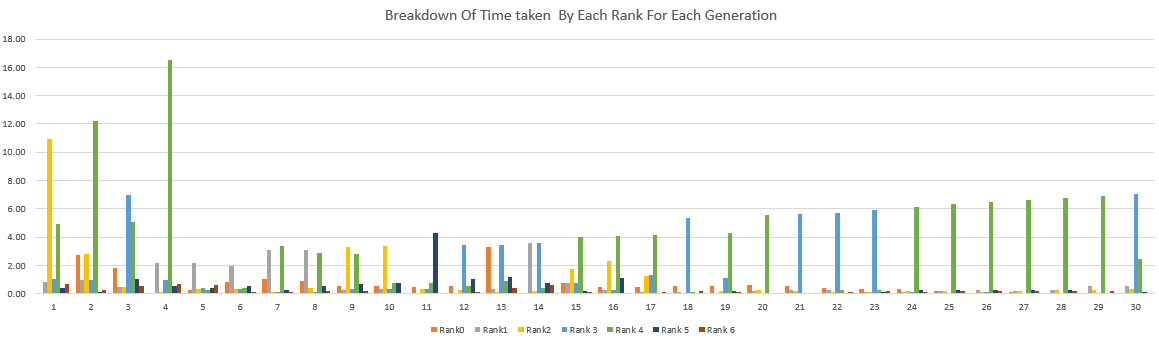
\includegraphics{./Images/Multiple-deme/rank_gen_timeTaken.PNG}
\caption{rankGenTime}
\end{figure}

Due to lower mutation chance, the parameters stay the same over
generations, thus keeping the fitness same. Comparing the same with
serial code as shown in figure below, it can be easily concluded that
time taken to train each network in parallel is less than the time taken
while training in sequential. The reason behind such behavior is
division and ease of access of RAM for each network. Keras add session
everytime a model is trained.

\begin{figure}[htbp]
\centering
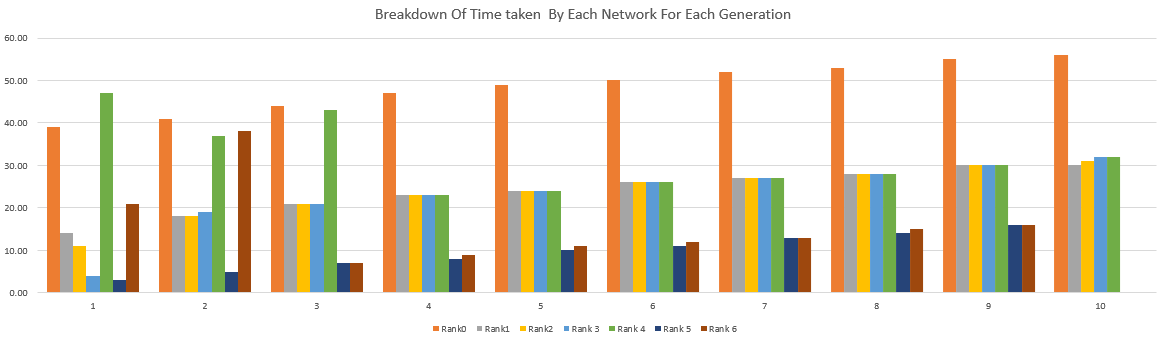
\includegraphics{./Images/Multiple-deme/rank_gen_timeTaken_Serial.PNG}
\caption{rank\_gen\_timeTaken\_Serial}
\end{figure}

The reduction of time at generation level is due to division of tasks in
parallel reducing the amount of time taken as per ``Law of division of
labor'', which can be seen below:
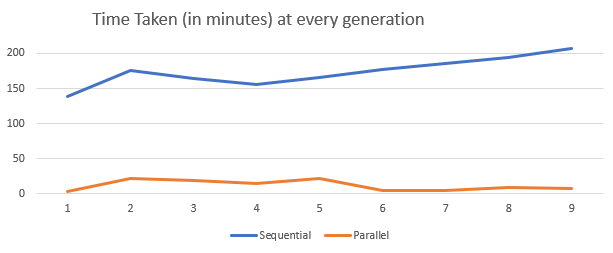
\includegraphics{./Images/Multiple-deme/timeS_vs_P.PNG}

Furthermore, an analysis on efficiency and speedups show the below:

\begin{longtable}[c]{@{}lllllllllll@{}}
\toprule
\begin{minipage}[b]{0.07\columnwidth}\raggedright\strut
Network
\strut\end{minipage} &
\begin{minipage}[b]{0.07\columnwidth}\raggedright\strut
Sequential Time
\strut\end{minipage} &
\begin{minipage}[b]{0.07\columnwidth}\raggedright\strut
Parallel Time
\strut\end{minipage} &
\begin{minipage}[b]{0.07\columnwidth}\raggedright\strut
Speedup
\strut\end{minipage} &
\begin{minipage}[b]{0.07\columnwidth}\raggedright\strut
Efficiency
\strut\end{minipage} &
\begin{minipage}[b]{0.07\columnwidth}\raggedright\strut
Best Accuracy - Serial
\strut\end{minipage} &
\begin{minipage}[b]{0.07\columnwidth}\raggedright\strut
Best Accuracy - Parallel
\strut\end{minipage} &
\begin{minipage}[b]{0.07\columnwidth}\raggedright\strut
Best Accuracy Generation - Serial
\strut\end{minipage} &
\begin{minipage}[b]{0.07\columnwidth}\raggedright\strut
Best Accuracy Generation - Parallel
\strut\end{minipage} &
\begin{minipage}[b]{0.07\columnwidth}\raggedright\strut
Time to reach best accuracy - serial
\strut\end{minipage} &
\begin{minipage}[b]{0.07\columnwidth}\raggedright\strut
Time to reach best accuracy - parallel
\strut\end{minipage}\tabularnewline
\midrule
\endhead
\begin{minipage}[t]{0.07\columnwidth}\raggedright\strut
-
\strut\end{minipage} &
\begin{minipage}[t]{0.07\columnwidth}\raggedright\strut
(time in minutes per generation)
\strut\end{minipage} &
\begin{minipage}[t]{0.07\columnwidth}\raggedright\strut
(time in minutes per generation)
\strut\end{minipage} &
\begin{minipage}[t]{0.07\columnwidth}\raggedright\strut
(Sequential time/Parallel time)
\strut\end{minipage} &
\begin{minipage}[t]{0.07\columnwidth}\raggedright\strut
(Speedup/Processor count)
\strut\end{minipage} &
\begin{minipage}[t]{0.07\columnwidth}\raggedright\strut
(in \%age)
\strut\end{minipage} &
\begin{minipage}[t]{0.07\columnwidth}\raggedright\strut
(in \%age)
\strut\end{minipage} &
\begin{minipage}[t]{0.07\columnwidth}\raggedright\strut
(generation number)
\strut\end{minipage} &
\begin{minipage}[t]{0.07\columnwidth}\raggedright\strut
(generation number)
\strut\end{minipage} &
\begin{minipage}[t]{0.07\columnwidth}\raggedright\strut
(time in h:mm)
\strut\end{minipage} &
\begin{minipage}[t]{0.07\columnwidth}\raggedright\strut
(time in h:mm)
\strut\end{minipage}\tabularnewline
\begin{minipage}[t]{0.07\columnwidth}\raggedright\strut
7
\strut\end{minipage} &
\begin{minipage}[t]{0.07\columnwidth}\raggedright\strut
139
\strut\end{minipage} &
\begin{minipage}[t]{0.07\columnwidth}\raggedright\strut
3
\strut\end{minipage} &
\begin{minipage}[t]{0.07\columnwidth}\raggedright\strut
46.3
\strut\end{minipage} &
\begin{minipage}[t]{0.07\columnwidth}\raggedright\strut
6.62
\strut\end{minipage} &
\begin{minipage}[t]{0.07\columnwidth}\raggedright\strut
48.4
\strut\end{minipage} &
\begin{minipage}[t]{0.07\columnwidth}\raggedright\strut
47.37
\strut\end{minipage} &
\begin{minipage}[t]{0.07\columnwidth}\raggedright\strut
1
\strut\end{minipage} &
\begin{minipage}[t]{0.07\columnwidth}\raggedright\strut
0
\strut\end{minipage} &
\begin{minipage}[t]{0.07\columnwidth}\raggedright\strut
1:08
\strut\end{minipage} &
\begin{minipage}[t]{0.07\columnwidth}\raggedright\strut
0:04
\strut\end{minipage}\tabularnewline
\begin{minipage}[t]{0.07\columnwidth}\raggedright\strut
70
\strut\end{minipage} &
\begin{minipage}[t]{0.07\columnwidth}\raggedright\strut
262
\strut\end{minipage} &
\begin{minipage}[t]{0.07\columnwidth}\raggedright\strut
29
\strut\end{minipage} &
\begin{minipage}[t]{0.07\columnwidth}\raggedright\strut
9
\strut\end{minipage} &
\begin{minipage}[t]{0.07\columnwidth}\raggedright\strut
0.13
\strut\end{minipage} &
\begin{minipage}[t]{0.07\columnwidth}\raggedright\strut
47.4
\strut\end{minipage} &
\begin{minipage}[t]{0.07\columnwidth}\raggedright\strut
45.47
\strut\end{minipage} &
\begin{minipage}[t]{0.07\columnwidth}\raggedright\strut
1
\strut\end{minipage} &
\begin{minipage}[t]{0.07\columnwidth}\raggedright\strut
5
\strut\end{minipage} &
\begin{minipage}[t]{0.07\columnwidth}\raggedright\strut
4:43
\strut\end{minipage} &
\begin{minipage}[t]{0.07\columnwidth}\raggedright\strut
8:18
\strut\end{minipage}\tabularnewline
\bottomrule
\end{longtable}

The accuracy that serial code taken hours to achieve can be gained in
minutes time running parallel code.

A comparison of fitness evolution with generations is drawn for various
ranks as shown below:
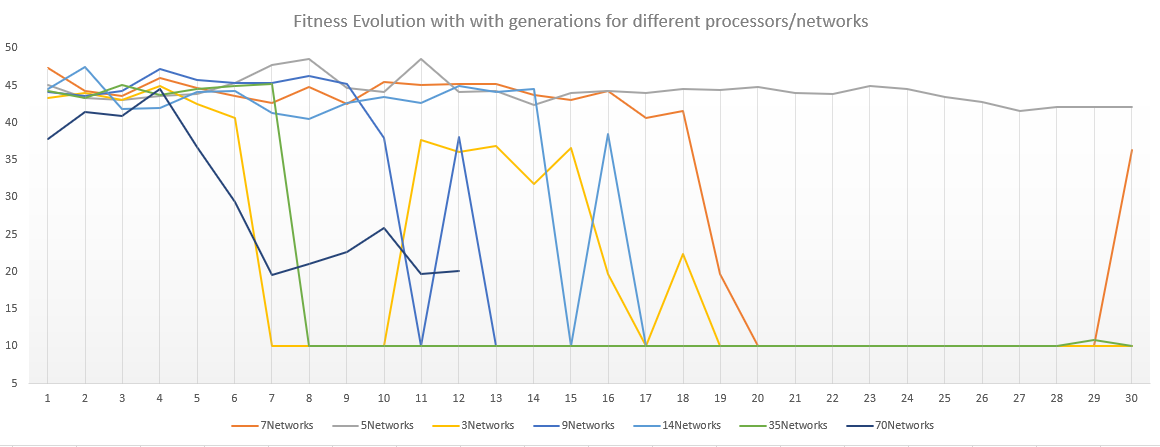
\includegraphics{./Images/Multiple-deme/fitnessEvolRanks.PNG}

This shows that increasing the number of ranks/networks has no impact on
fitness, however, increasing the ranks for the analysis does help in
getting the fitness sooner.

\begin{longtable}[c]{@{}lllll@{}}
\toprule
\begin{minipage}[b]{0.17\columnwidth}\raggedright\strut
Processors
\strut\end{minipage} &
\begin{minipage}[b]{0.17\columnwidth}\raggedright\strut
Number of Islands
\strut\end{minipage} &
\begin{minipage}[b]{0.17\columnwidth}\raggedright\strut
Population per Island
\strut\end{minipage} &
\begin{minipage}[b]{0.17\columnwidth}\raggedright\strut
Best Fitness
\strut\end{minipage} &
\begin{minipage}[b]{0.17\columnwidth}\raggedright\strut
Time (in minutes)
\strut\end{minipage}\tabularnewline
\midrule
\endhead
\begin{minipage}[t]{0.17\columnwidth}\raggedright\strut
7
\strut\end{minipage} &
\begin{minipage}[t]{0.17\columnwidth}\raggedright\strut
3
\strut\end{minipage} &
\begin{minipage}[t]{0.17\columnwidth}\raggedright\strut
3
\strut\end{minipage} &
\begin{minipage}[t]{0.17\columnwidth}\raggedright\strut
41.48
\strut\end{minipage} &
\begin{minipage}[t]{0.17\columnwidth}\raggedright\strut
17
\strut\end{minipage}\tabularnewline
\begin{minipage}[t]{0.17\columnwidth}\raggedright\strut
14
\strut\end{minipage} &
\begin{minipage}[t]{0.17\columnwidth}\raggedright\strut
5
\strut\end{minipage} &
\begin{minipage}[t]{0.17\columnwidth}\raggedright\strut
3
\strut\end{minipage} &
\begin{minipage}[t]{0.17\columnwidth}\raggedright\strut
10
\strut\end{minipage} &
\begin{minipage}[t]{0.17\columnwidth}\raggedright\strut
11min
\strut\end{minipage}\tabularnewline
\begin{minipage}[t]{0.17\columnwidth}\raggedright\strut
21
\strut\end{minipage} &
\begin{minipage}[t]{0.17\columnwidth}\raggedright\strut
3
\strut\end{minipage} &
\begin{minipage}[t]{0.17\columnwidth}\raggedright\strut
7
\strut\end{minipage} &
\begin{minipage}[t]{0.17\columnwidth}\raggedright\strut
10
\strut\end{minipage} &
\begin{minipage}[t]{0.17\columnwidth}\raggedright\strut
3min
\strut\end{minipage}\tabularnewline
\bottomrule
\end{longtable}

From the above table it can be inferred that implementation of the
island model did not result in better fitness

\end{document}
